 \documentclass[aps,prb,groupedaddress,showpacs,twocolumn,superscriptaddress,10pt]{revtex4-2}

\setlength{\paperheight}{11in}

\usepackage{graphicx}
\usepackage{mathtools}
\usepackage{amsmath}
\usepackage{amssymb}
\usepackage{bbm}
\usepackage{bm}
\usepackage{cancel}
\usepackage{xspace}
\usepackage{braket}
\usepackage{xcolor}   
\usepackage{calrsfs}
\usepackage{comment}
\usepackage{placeins}%enables \FloatBarier
\usepackage{hyperref}


\usepackage{units}
 
\synctex=1

\DeclareMathAlphabet{\pazocal}{OMS}{zplm}{m}{n} % capital letters for Re and Im parts 
\newcommand{\capcali}{\pazocal{I}}
\newcommand{\capcalr}{\pazocal{R}}

\newcommand{\ee}{\mathrm{e}}  % Euler number 
\DeclareMathOperator*{\ii}{i} % imaginary unit
\newcommand*\dd{\mathop{}\!\mathrm{d}}

\renewcommand{\vec}[1]{\bm{#1}} % vectors in bold
\newcommand{\mat}[1]{\bm{#1}} % matrices in bold 
\newcommand{\kel}[1]{\underline{#1}} % objects on Keldysh contour

\newcommand{\defeq}{\overset{\mathrm{def}}{=\joinrel=}} % definition symbol ":="  
 
%% REFERENCE
\newcommand{\fig}[1]{Fig.\thinspace{}\ref{#1}}
\newcommand{\figs}[1]{Figs.\thinspace{}\ref{#1}} 
\newcommand{\Fig}[1]{Figure \ref{#1}}
\newcommand{\eq}[1]{Eq.\thinspace{}(\ref{#1})}
\newcommand{\Eq}[1]{Eq.\thinspace{}(\ref{#1})}
\newcommand{\eqs}[1]{Eqs.\thinspace{}(\ref{#1})}
\newcommand{\Eqs}[1]{Eqs.\thinspace{}(\ref{#1})}
\newcommand{\feqs}{eqs.\@\xspace}
\newcommand{\fEqs}{Eqs.\@\xspace}
\newcommand{\ch}{Ch.\@\xspace}
\newcommand{\Ch}{Ch.\@\xspace}
\newcommand{\pa}{par.\@\xspace}
\newcommand{\Pa}{Par.\@\xspace}
\newcommand{\se}{Sec.\@\xspace}
\newcommand{\Se}{Sec.\@\xspace}
\newcommand{\app}{App.\@\xspace}
\newcommand{\App}{App.\@\xspace}

%% CITE
\newcommand{\etal}[0]{\textit{et al.}}
\newcommand{\tcite}[1]{Ref.~~\cite{#1}}
\newcommand{\tcites}[1]{Refs.~~\cite{#1}}
\newcommand{\Tcite}[1]{Ref.~~\cite{#1}}
\newcommand{\Tcites}[1]{Refs.~~\cite{#1}}


%Defs
\newcommand{\und}{\underline}
\newcommand{\iim}{\Im{}\,}
\newcommand{\li}{\mathcal L}
\newcommand{\ga}[1]{\Gamma^{(#1)}}
\newcommand{\up}{\ensuremath{\uparrow}}
\newcommand{\dw}{\ensuremath{\downarrow}}
\newcommand{\vv}[1]{\boldsymbol{#1}}
\newcommand{\Dph}{\underline{\Delta}_\mathrm{ph}(\omega)}
\newcommand{\Daux}{\underline{\Delta}_\mathrm{aux}(\omega)}
\newcommand{\DRph}{\Delta^R_\mathrm{ph}(\omega)}
\newcommand{\DRaux}{\Delta^R_\mathrm{aux}(\omega)}
\newcommand{\DKph}{\Delta^K_\mathrm{ph}(\omega)}
\newcommand{\DKaux}{\Delta^K_\mathrm{aux}(\omega)}

 
%choose
%\newcommand{\phys}{\text{phys}}
%\newcommand{\phys}{\text{DMFT}}
\newcommand{\phys}{} %my preference 
 
 
\def\bra#1{\mathinner{\langle{#1}|}}
\def\ket#1{\mathinner{|{#1}\rangle}}
\def\braket#1{\mathinner{\langle{#1}\rangle}}
\def\Bra#1{\left<#1\right|}
\def\Ket#1{\left|#1\right>}

\newcommand{\nag}{{\phantom{\dagger}}} 

\newcommand{\pim}{IM$_\mathrm{ph}$ }
\newcommand{\aim}{IM$_\mathrm{aux}$ }
\newcommand{\pimns}{IM$_\mathrm{ph}$} 
\newcommand{\aimns}{IM$_\mathrm{aux}$}

\newcommand{\mscomm}[1]{{\color{blue} MS Comment: #1}}
%\newcommand{\kh}[1] {\textcolor{green}{KH comment: #1}}

\definecolor{orange}{RGB}{252,77,6}
\definecolor{brown}{RGB}{200,127,50}

\definecolor{ao(english)}{rgb}{0.0, 0.5, 0.0}

\newcommand{\pgcomm}[1]{{\color{ao(english)} [PG COMMENT: #1]}}
\newcommand{\pgch}[1]{{\color{ao(english)} #1}}
  
 
\begin{document}

\title{Impact ionization processes in driven Mott insulating layer: influence of fermion baths and phonons}

\author{Paolo Gazzaneo}
\email[]{paolo.gazzaneo@tugraz.at}
\affiliation{Institute of Theoretical and Computational Physics, Graz University of Technology, 8010 Graz, Austria}
\author{Tommaso Maria Mazzocchi}
\affiliation{Institute of Theoretical and Computational Physics, Graz University of Technology, 8010 Graz, Austria}
\author{Jan Lotze}
\affiliation{Institute of Theoretical and Computational Physics, Graz University of Technology, 8010 Graz, Austria}
\author{Enrico Arrigoni}
\email[]{arrigoni@tugraz.at}
\affiliation{Institute of Theoretical and Computational Physics, Graz University of Technology, 8010 Graz, Austria}

\date{\today}
 
\begin{abstract}   

We study a model for photovoltaic energy collection consisting of a Mott insulating layer coupled to local acoustic phonons between two wide-band fermion baths at different chemical potentials, driven to the non-equilibrium steady state by an external AC field. We treat electron correlations with non-equilibrium dynamical mean field theory (DMFT) using the so-called auxiliary master equation approach as impurity solver, incuding phonons via the Migdal approximation. 
 
We show that with a small coupling to fermion baths, the peak of the photocurrent is mainly due to impact ionization processes, while with higher coupling is due primarily to direct excitations. This occurs also for higher electric field amplitudes, that boost overall the photocurrent and the double occupation. Acoustic phonons slightly enhance the photocurrent for small driving frequencies and suppress it at higher values, in correspondence to the peak, disregarding the dominant electronic scattering process taking place. Their effect is independent of the bath-layer coupling value and the electric field amplitude.  
  
\end{abstract}

% insert suggested PACS numbers in braces on next line
%71.10.-w Theories and models of many-electron systems
%71.15.-m Methods of electronic structure calculations
%71.27+a Strongly correlated electron systems; heavy fermions
% 71.38.−k Polarons and electron-phonon interactions
% 72.20.Jv Charge carriers: generation, recombination, lifetime, and trapping
% 73.21.−b Electron states and collective excitations in multilayers, quantum wells, mesoscopic, and nanoscale systems
%73.21.La Quantum dots (Electron states and collective excitations in multilayers, quantum wells, mesoscopic, and nanoscale systems)
% 73.50.Pz Photoconduction and photovoltaic effects
\pacs{71.10.Fd,71.15.-m,71.27+a,71.38.-k,72.20.Jv,73.21.-b,73.21.La,73.50.Pz}
       
\maketitle   


\section{Introduction} 
\label{sec:intro} 

\pgcomm{IS FERMION BATHS THE APPROPRIATE TERM?}
 
 
The idea of designing photovoltaic devices exploiting the Mott gap to convert electromagnetic radiation into energy has become popular in the recent years \cite{mano.10,li.ch.13,gu.gu.13,co.ma.14,wa.li.15}. In particular, it has been
suggested that in strongly correlated materials, highly excited charge carriers could use their extra energy to excite additional carriers across the Mott gap via impact ionization \cite{mano.10,co.ma.14}, thus
potentially improving their efficiency beyond the Shockley-Queisser limit \cite{sh.qu.61}. Although impact ionization is also present in conventional semiconductor devices, the time scales for electron-electron scattering are typically much longer than in correlated materials, so that highly excited electrons will mostly dissipate their energy to phonons. 

Experimentally, evidence for fast carrier multiplication processes has indeed been detected via pump-probe experiments in VO$_2$ \cite{ho.bi.16}. Oxide heterostructures based on LaVO$_3$/SrTiO$_3$ have been identified as promising candidates, due to the ideal band gap and the strong polar field, able to separate the excited charge carriers \cite{as.bl.13}. There are however some drawbacks, such as the low mobility of the carriers \cite{wa.li.15,je.re.18}, which still question these materials’ applicability as efficient solar cells. In this regard, it has to be mentioned that, while a large-scale application of Mott-based solar cells may be hard to achieve, the employment of such systems as photodetectors may be more promising on the long run, due to their high photoresponsivity. 

Therefore, the properties of the Mott-based photovoltaic mechanism deserve to be investigated further, from the scientific point of view and for future applications in order to explore, whether alternative unexpected paths could be opened. And in fact, a lot of theoretical work has been done, in order to understand the impact ionization process (see, e.g. \cite{co.ma.14,ec.we.11,ec.we.13,we.he.14,pe.be.19,so.do.18,ka.wo.20,ma.ev.22}). 

The effects of the coupling to metallic leads and of phonons dissipation are essential features to properly establish the occurrence of impact ionization in Mott-based photovoltaic setups. They haven't been taken into account up to now and in this article we address such issues.

 
% First, because the effect of phonons on impact ionization is still to clarify completely and therefore there are still questions regarding the physical mechanisms to be answered. Once such questions are answered, a more detailed treatment of phonons, together with DFT may address more accurately the precise entity of the their effect.
 
\begin{figure}[ht]
% \captionsetup{width=\textwidth} 
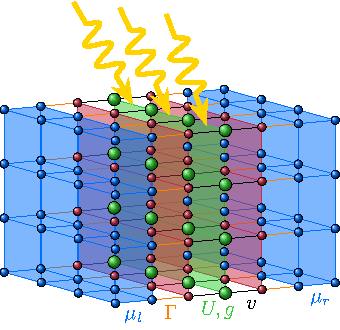
\includegraphics[width=0.9\linewidth]{./figures_Paper1/setup.pdf}
\caption{(Colour online) Schematic representation of the considered setup. A correlated layer with local Hubbard interaction $U$ and electron-phonon coupling $g$ (green) is sandwiched between two non-interacting layers (red) via the coupling $v$ (black). The latter are in turn coupled via $\Gamma$ (orange) to wide-band fermion reservoirs (blue) at different chemical potentials $\mu_{l/r}$.}
\label{fig:setup}
\end{figure}   
 
The setup used is depicted in Fig.\ref{fig:setup}: a Hubbard insulating layer with local acoustic phonons under AC driving is put between two intermediate non-interacting layers coupled to wide-band fermion reservoirs at different chemical potentials, acting as metallic leads. For sake of simplicity, we refer for the rest of the article to the non-interacting layers and fermion reservoirs together simply as fermion baths. We address the non-equilibrium steady state situation under an external AC field, treated via nonequilibrium Floquet dynamical mean-field theory (F-DMFT). 

Our goal is to show for which values of the bath-layer coupling impact ionization clearly occurs and how is influenced by the effect of phonons. 

We limit our analysis to qualitative and semi-quantitative features of the influence of fermion baths and phonons on photocurrent, double occupation and spectral properties. 
An accurate quantitative analysis of such effects and their relative signatures in possible experimental setups of Mott solar cells is outside the scope of this work. 
     

We find that a small coupling to fermion baths clearly enhances impact ionization respect to a bigger coupling, for which direct excitations are dominant. Impact ionization therefore plays a crucial role, compensating the smaller charge injection and giving the same magnitude in the photocurrent of the case with a bigger coupling. Such results remain the same considering higher values of electric field amplitude, although the current and double occupation are greatly increased. The phonons slightly enhance the photocurrent for small driving frequencies, while suppressing it at higher values, in corrispondence to the peak, disregarding the dominant electron scattering process taking place. Such influence of phonons on the photocurrent is substantially unaltered sweeping over different values of the bath-layer coupling and of electric field amplitude.  

The structure of the paper is the following: in Sec.\ref{sec:Model} we describe the model Hamiltonian. Methods, formalism and observables used are explained in Sec.\ref{sec:Method_formalism}. We discuss our results in Sec.\ref{sec:results}. We present our conclusions in Sec.\ref{sec:conclusions}. 
 
  
\section{Model}
\label{sec:Model}

Our setup (Fig.\ref{fig:setup}) consists of a central Hubbard layer at half filling with local phonon coupling, under an external AC driving,attached to fermionic baths: 

\begin{equation}
\label{eq:Hamiltonian}
\begin{split} 
\hat{H}(t)&=\varepsilon_c \sum_{i\sigma}\hat{n}_{i\sigma} -\sum_{\sigma}\sum_{(i,j)} t_{ij}(t) \hat{c}^{\dagger}_{i\sigma} \hat{c}_{j\sigma}
\\ & + U \sum_{i} \hat{n}_{i\uparrow} \hat{n}_{i\downarrow}+\hat{H}_{e-ph} + \hat{H}_{ph}+\hat{H}_{bath}
\end{split}
\end{equation} 

The operator $\hat{c}^{\dagger}_{i\sigma}$ ($\hat{c}_{i\sigma}$) creates (annihilates) an electron with spin $\sigma= \lbrace \uparrow,\downarrow \rbrace$ on the \emph{i-th} lattice site, with $\hat{n}_{i\sigma}\equiv \hat{c}^{\dagger}_{i\sigma} \hat{c}_{i\sigma}$. We denote with $(i,j)$ the sum over next neighbour sites and with $\varepsilon_c \equiv -U/2$ the electron onsite energy. The AC field consists of a time-periodic, homogeneous and monochromatic electric field with frequency $\Omega$. It enters via the Peierl's substitution in the time-dependent hopping in Eq. (\ref{eq:Hamiltonian}) \cite{peie.33}:
\begin{equation}\label{eq:peierls} 
t_{ij}(t) = t_{c} \ e^{-i \frac{q}{\hbar} \left( \vec{r}_j - \vec{r}_i \right) \cdot \vec{A}(t)}, 
\end{equation} 
where $t_{c}$ is the intra-lattice hopping, $\vec{A}$(t) is the time-dependent vector potential, $\hbar$ the Planck's constant and $q$ the charge of the electron. Here $\vec{A}(t)=\vec{e}_{0} A(t)$ is along the lattice body diagonal, i.e. $\vec{e}_{0}=(1,1,\dots,1)$. For the AC field, $A(t)=\frac{\hbar}{qa}A\sin\Omega t$, with $A=-\frac{qE_0a}{\hbar\Omega}$, being $E_0$ the electric field amplitude and $a$ the lattice spacing ~\cite{ts.ok.08}. Therefore in the temporal gauge $\vec{E}= -\partial_{t}\vec{A}(t) = \vec{e}_{0}E_0 \cos\Omega t$.
  
The local electron-phonon coupling is included as in Ref.\cite{ma.ga.22u}, considering an acoustic phonon branch attached to each lattice site via the Hamiltonian 
\begin{equation}\label{eq:e-ph_ham} 
\hat{H}_{e-ph} = g \sum_{i\sigma} \hat{n}_{i\sigma} \hat{x}_{i},  
\end{equation}
with $g$ the electron-phonon coupling and $\hat{x}_{i} \equiv \frac{1}{\sqrt{2}} \left( \hat{b}^{\dagger}_{i} + \hat{b}_i \right)$, where $\hat{b}^{\dagger}_{i}$ ($\hat{b}_{i}$) creates (annihilates) a phonon of the acoustic branch at site $i$, with dispersion relation in $\hat{H}_{ph}$ \cite{ma.ga.22u}.  
 
Details on the baths are provided in \ref{sec:Dyson_equation}. 
 
In this paper we consider the correlated system as a $d$-dimensional layer in $d+1$ dimensions and we take the limit of infinite dimensions $d \rightarrow \infty$ by rescaling the hopping as $t_{c}=t^{*}/2\sqrt{d}$ \footnote{We tune $t^*$ such that we reproduce as best as possible the DOS of a 2D layer with $t_c$ = 1, following Ref.\cite{so.do.18}.}. With $a=1$, sums over crystal momentum ${\bf k}$ of a generic quantity $\chi$ read $\sum_{{\bf k}} \chi(\omega,{\bf k}) \rightarrow \int d\epsilon \int   d\overline{\epsilon} \ \rho(\epsilon,\overline{\epsilon}) \chi(\omega;\epsilon,\overline{\epsilon})$ with $\rho(\epsilon,\overline{\epsilon}) = (1/\pi t^{* 2}) \ exp(-( \epsilon^{2} + \overline{\epsilon}^{2})/t^{* 2})$ the joint density of states (JDOS) ~\cite{ts.ok.08}, with  
\begin{align}\label{eq:d-dim_crystal_dep}
\begin{split}  
\epsilon & = -2t_{c} \sum_{i=1}^{d} cos(k_i a) \\  
\overline{\epsilon}& = -2t_{c}\sum_{i=1}^{d} sin(k_i a). \\
\end{split}  
\end{align}   
 
In this paper we set $\hbar = k_B = a = 1 = -q$, so that every physical quantity is in units of $t^{*}$.
	  
\section{Method and formalism}    
\label{sec:Method_formalism}  

\subsection{Floquet Green's Function method}   
\label{sec:GFs_Dyson_Floquet}
 
 
	 
To correctly describe the nonequilibrium periodic steady-state (NESS), we use the Floquet generalization of non-equilibrium Green's function (NEGF) approach \cite{ts.ok.08}. Every function $G(t;t{'})$ satisfying the periodicity relation $G(t;t{'})=G(t+\tau;t{'}+\tau)$, with $\tau=2\pi/\Omega$ the period related to the external driving frequency $\Omega$, may be represented as \cite{ts.ok.08,sc.mo.02u,jo.fr.08}

\begin{equation}
\label{eq:FloquetGF} 
\underline{G}_{mn}(\omega) =\int dt_{rel} \int_{-\tau/2}^{\tau/2} \frac{dt_{av}}{\tau} e^{i[\left(\omega+m\Omega\right) t -\left( \omega+n\Omega\right)t{'}]} \underline{G}(t,t'),
\end{equation}

known as the the \emph{Keldysh-Floquet} GF, and

\begin{equation}\label{eq:WignerGF}
\underline{G}_{l}(\omega) =\int dt_{rel} \int_{-\tau/2}^{\tau/2} \frac{dt_{av}}{\tau} e^{i\omega t_{rel} + il\Omega t_{av}} \underline{G}(t,t'),
\end{equation}

the \emph{Wigner} GF ~\cite{ts.ok.08}. $t_{rel} = t-t{'}$ and $t_{av} = (t+t{'})/2$ are the relative and average-time variables. Eqs. (\ref{eq:FloquetGF}) and (\ref{eq:WignerGF}) are related via the relation

\begin{equation}\label{eq:Wig2Fl}
\underline{G}_{mn}(\omega)=\underline{G}_{m-n}\left(\omega+\frac{m+n}{2}\Omega \right),
\end{equation}

We denote in the rest of this work a Floquet-represented matrix as either $X_{mn}$, with the explicit indices, or using a boldface letter, $\bf{X}$. A single index as subscript, $X_{l}$, is reserved for the Wigner representation. The underline indicates the overall structure 
\begin{equation}\label{eq:Keld-structure}
\underline{{\bf G}} \equiv 
\begin{pmatrix}
{\bf G}^{R} & {\bf G}^{K}\\
{\bf 0}         & {\bf G}^{A} \\
\end{pmatrix},
\end{equation}

which contains the \emph{retarded}, \emph{advanced} and \emph{Keldysh} components $\textbf{G}^{\text{R,A,K}}$, where $\textbf{G}^{\text{A}}=(\textbf{G}^{\text{R}})^{\dagger}$. The \emph{Keldysh} component is defined as $\textbf{G}^{K} \equiv \textbf{G}^{>} + \textbf{G}^{<}$, with $\textbf{G}^{\lessgtr}$ the \emph{lesser} and \emph{greater} components~\cite{schw.61,keld.65,ra.sm.86,ha.ja}
 
\subsection{Dyson equation}
\label{sec:Dyson_equation}
	 
	 
The lattice Floquet GF of our setup obeys the Dyson equation 

\begin{equation}\label{eq:FullDysonEq}
\underline{{\bf G}}^{-1}(\omega_n;\epsilon,\overline{\epsilon}) = \underline{{\bf G}}^{-1}_{0}(\omega_n;\epsilon,\overline{\epsilon}) - \underline{{\bf \Sigma}}(\omega_n;\epsilon,\overline{\epsilon}) - \underline{{\bf \Sigma}}_{e-ph}(\omega_n;\epsilon,\overline{\epsilon}),
\end{equation}
  
The lattice GF of the non-interacting part of the Hamiltonian, Eq. (\ref{eq:Hamiltonian}), is 
 
\begin{equation}\label{eq:non-int_InvGF} 
\underline{G}^{-1}_{0,mn}(\omega_n;\epsilon,\overline{\epsilon}) =  \underline{g}^{-1}_{0,mn}(\omega_n;\epsilon,\overline{\epsilon}) - \sum_{\rho\in\{l,r\}}v^2_{\rho}\underline{g}_{b,\rho}(\omega_n;\epsilon)\delta_{mn},
\end{equation}

 with $v_{l/r}$ the bath-layer coupling, $\omega_n \equiv \omega + n\Omega$, $n\in\mathbbm{Z}$, and 

 \begin{align}\label{eq:inv_non-int_lat_GF_comps}
\begin{split}
\left[ g^{-1}_{0}(\omega_n;\epsilon,\overline{\epsilon})) \right]^{R}_{mn} & = \left( \omega_n + i0^{+} -\varepsilon_c \right)\delta_{mn} - \varepsilon_{mn}(\epsilon,\overline{\epsilon})) \\
\left[ g^{-1}_{0}(\omega_n;\epsilon,\overline{\epsilon})) \right]^{K}_{mn} & = 0 \\
\end{split}.
\end{align}

In the steady-state, the inverse Keldysh component is negligible \cite{so.do.18}. The Floquet dispersion relation, $\varepsilon_{mn}$, for the AC field in a hyper-cubic lattice is \cite{ts.ok.08} 
 
\begin{equation}
\label{eq:Floquet_disp}
\varepsilon_{mn}(\epsilon,\overline{\epsilon}) = \left\{
                \begin{array}{ll}
                  \epsilon J_{m-n}(A) \quad m-n:\textrm{even} \\
                  i\overline{\epsilon}J_{m-n}(A) \quad m-n:\textrm{odd}
                \end{array}
              \right  .
\end{equation} 

with $J_n$ denoting the $n$-th order Bessel function of the first kind, with argument $A$ defined in \se\ref{sec:Model}.  $\underline{g}_{b,l/r}$ is the GF of the bath, composed by a $d$-dimensional layer, coupled to an infinite fermion reservoir via the hopping term $\Gamma$ (see Fig.\ref{fig:setup}). 
Its \emph{retarded} and \emph{Keldysh} components are 

\begin{equation}
\label{eq:retarded_bath_GF}
g^{R}_{b,l/r}(\omega;\epsilon) = \frac{1}{\omega-\varepsilon_{l/r}(\epsilon)+i\Gamma_{l/r}}
\end{equation}


\begin{equation}
\label{eq:keldysh_bath_GF}
g^{K}_{b,l/r}(\omega;\epsilon) = 2i \Im g_{b,l/r}^{R}(\omega;\epsilon)[1-2f(\omega,\mu_{l/r},\beta)]
\end{equation} 

with dispersion $\varepsilon_{l/r}(\epsilon)=\varepsilon_{l/r} +\frac{t_{l/r}}{t^*}\epsilon$, where $f(\omega,\mu_{l/r},\beta)=1/(\ee^{\beta(\omega-\mu_{l/r})}+1)$ is the Fermi-Dirac distribution function at inverse temperature $\beta \equiv 1/T$, $\varepsilon_{l/r}$ is the onsite energy and $t_{l/r}$ is the hopping within the $d$-dimensional layer of the bath. 
 


The electron self-energy (SE) $\underline{\bf{\Sigma}}$ is obtained from F-DMFT and is therefore independent of the crystal momentum, i.e., $\underline{\bf{\Sigma}}(\omega;\epsilon,\overline{\epsilon}) \simeq \underline{\bf{\Sigma}}(\omega)$. Further details are given in Sec. \ref{sec:FDMFT_implementation}. 

The e-ph SE is also included locally, $\underline{\bf{\Sigma}}_{e-ph}(\omega;\epsilon,\overline{\epsilon}) \simeq \underline{\bf{\Sigma}}_{e-ph}(\omega)$. In terms of the contour time arguments $z,z^\prime$ it has the form

\begin{equation}\label{eq:backbone_e-ph_SE}
\Sigma_{\text{e-ph}}(z,z^{\prime}) = ig^{2} G(z,z^{\prime}) D_{\text{ph}}(z,z^{\prime}).
\end{equation}

The Keldysh components ~\cite{ao.ts.14} of the non-interacting phonon GF $\kel{D}_{\text{ph}}(t,t^{\prime})$ are given by
\begin{align}\label{eq:Ph_Prop_time}
\begin{split} 
D^{\text{R}}_{\text{ph}}(t,t^{\prime}) & = -i \theta(t-t^{\prime}) \int \dd\omega \ \ee^{-i\omega\left(t-t^{\prime}\right)} A_{\text{ph}}(\omega), \\
D^{>}_{\text{ph}}(t,t^{\prime}) & = -i \int \dd\omega \ \ee^{-i\omega\left(t-t^{\prime}\right)} A_{\text{ph}}(\omega) \left( 1 + b(\omega) \right) \\
D^{<}_{\text{ph}}(t,t^{\prime}) & = -i \int \dd\omega \ \ee^{-i\omega\left(t-t^{\prime}\right)} A_{\text{ph}}(\omega) \ b(\omega), \\
\end{split},
\end{align}
where $b(\omega)=1/(\ee^{\beta\omega}-1)$ is the Bose-Einstein distribution function at inverse temperature $\beta$. We focus on acoustic phonons, with $A_{\text{ph}}(\omega) = \omega/(\omega^{2}_{\text{ph}}) \ee^{-| \omega|/\omega_{\text{ph}}}$ the phonon spectral function and $\omega_{\text{ph}}$ a soft cutoff frequency \cite{pi.li.21}. The retarded and Keldysh components of Eq.~\eqref{eq:backbone_e-ph_SE} can be found in Ref.\cite{ma.ga.22u}.
 
	
\subsection{Floquet DMFT}
\label{sec:FDMFT_implementation}
 

We compute the electron SE in the Dyson equation Eq.\eqref{eq:FullDysonEq} using DMFT approach~\cite{me.vo.89,ge.ko.92,ge.ko.96}, and in particular its nonequilibrium Floquet (F-DMFT) extension~\cite{ts.ok.08,sc.mo.02u,jo.fr.08}. \pgcomm{(I CAN CANCEL IT MAYBE, UNUSEFUL?) The DMFT approximation consists in neglecting the crystal momentum dependence of the electron SE, i.e. $\kel{\mat{\Sigma}}(\omega,\epsilon,\overline{\epsilon}) \to \kel{\mat{\Sigma}}(\omega)$. This allows us to map the original problem into a single-site impurity model with a bath hybridization function, $\kel{\mat\Delta}(\omega)$ encoding the effect of all other lattice sites.} We briefly describe now the self-consistent F-DMFT scheme used.
(i) We start from an initial guess for electron SE $\kel{\mat{\Sigma}}(\omega)$. (ii) We compute the local electron Green's function as 

\begin{equation}\label{eq:Lat_LocGF}
\begin{split}
\kel{\mat G}_{\text{loc}}(\omega) &= \int \dd\epsilon \int \dd\overline{\epsilon} \ \rho(\epsilon,\overline{\epsilon}) \times \\ 
&\times \left[ \left( \kel{\mat G}^{-1}_{0}(\omega,\epsilon,\overline{\epsilon}) - \kel{\mat\Sigma}(\omega) - \kel{\mat \Sigma}_{\text{e-ph}}(\omega) \right)^{-1} \right].
\end{split}
\end{equation}	

(iii) We compute $\kel{\mat{\Sigma}}_{\text{e-ph}}(\omega)$
from Eq.\eqref{eq:backbone_e-ph_SE}.
(iv) We map the problem into a in a single-site impurity one, with $\kel{\mat\Delta}(\omega)$ given by 

\begin{equation}\label{eq:imp_Dyson_eq}
\kel{\mat{\Delta}}(\omega) = \kel{\mat{g}}^{-1}_{\text{0,site}}(\omega) - \kel{\mat{G}}^{-1}_{\text{loc}}(\omega) - \kel{\mat{\Sigma}}(\omega)
\end{equation}

where $\kel{\mat{g}}^{-1}_{\text{0,site}}(\omega)$ is defined as in Eq.~(\ref{eq:inv_non-int_lat_GF_comps}) but without $\varepsilon_{mn}(\epsilon,\overline{\epsilon})$. (v) We map the impurity problem to an auxiliary one, we solve the many body problem and determine the new $\kel{\mat{\Sigma}}(\omega)$(see \ref{sec:amea}). (vi) We plug the obtained SEs in step (ii) and we iterate the steps (ii)-(vi) until convergence.


\subsubsection{Floquet-diagonal self-energy approximation}
\label{sec:FDSA}
   

Eq.\eqref{eq:imp_Dyson_eq} gives a periodic time-dependent bath hybridization function $\kel{\mat\Delta}(\omega)$. We want to address photovoltaic effects, therefore following Ref.\cite{so.do.18}, we consider only the $(0,0)$-Floquet matrix element of Eq.\eqref{eq:imp_Dyson_eq} (corresponding to the time-average over a period $\tau$) and  we employ the Floquet-diagonal self-energy approximation (FDSA) for $\kel{\mat{\Sigma}}(\omega)$.  We employ the FDSA in Eq.\eqref{eq:FullDysonEq} also for $\underline{\bf{\Sigma}}_{e-ph}(\omega)$, namely $\kel{\Sigma}_{mn,e-ph}(\omega_n) = \kel{\Sigma}_{00,e-ph}(\omega_n)\delta_{mn}$ \footnote{In the range in which FDSA is justified for $\kel{\Sigma}$, $\kel{\Sigma}_{00,e-ph}$ is orders of magnitude bigger than the other Floquet matrix elements $\kel{\Sigma}_{mn,e-ph}$.}.  Therefore Eq.\eqref{eq:imp_Dyson_eq} reads  

\begin{equation}\label{eq:imp_Dyson_eq_av}
\kel{\Delta}(\omega) = \kel{g}^{-1}_{\text{0,site}}(\omega) - \kel{G}^{-1}_{\text{loc}}(\omega) - \kel{\Sigma}(\omega)
\end{equation}

where all the quantities are time-averaged. Once we obtain the new $\kel{\Sigma}(\omega)$, we reconstruct the Floquet dependence of SEs via the translation property $\kel{\Sigma}_{mn}(\omega) = \kel{\Sigma}_{00}(\omega+m\Omega)\delta_{mn}$.  
	  
\subsubsection{Auxiliary master equation approach}
\label{sec:amea}


We briefly summarize the impurity solver used in step (v) of DMFT self-consistent loop (Sec.\ref{sec:FDMFT_implementation}). 

We solve the many-body problem using the auxiliary master equation approach (AMEA)~\cite{ar.kn.13,do.nu.14,do.ga.15,do.so.17}. It maps the impurity problem in an open quantum system consisting of a finite number of bath sites $N_{\text{B}}$ attached to Markovian reservoirs described by the Lindblad equation. The corresponding hybridization function $\kel{\Delta}_{\text{aux}}(\omega)$ is obtained by fitting the original DMFT one. We reach convergence once $\kel{\Delta}_{\text{aux}}$ agrees with $\kel{\Delta}$ with a sufficient accuracy. With the parameters obtained from $\kel{\Delta}_{\text{aux}}$, we solve the auxiliary problem using standard many-body-diagonalization methods for open quantum systems, obtaining the new $\kel{\Sigma}(\omega)$. 
	
\subsection{Observables}
\label{sec:observables}  
 
	  
In this article, we consider time-averaged observables, defined as follows.

The photocurrent (or simply current, without any ambiguity) flowing from the left fermion bath to the right one, passing through the correlated layer is given by 


\begin{align}
 j_{L\rightarrow R}&=v^2\int_{-\frac{\Omega}{2}}^{\frac{\Omega}{2}}\frac{d\omega}{2\pi} \int d\epsilon \int d\overline{\epsilon} \rho(\epsilon,\overline{\epsilon}) \text{Re Tr} \boldsymbol{J}\label{eq: Current furmula_Omega}\\
  &= v^2\int_{-\infty}^{+\infty}\frac{d\omega}{2\pi} \int d\epsilon \int d\overline{\epsilon} \rho(\epsilon,\overline{\epsilon}) \text{Re} J_{00}\label{eq: Current furmula_00}
  \end{align} 
where $\boldsymbol{J}$ is given by the following expression
\begin{equation}
  \boldsymbol{J}=\left[\boldsymbol{G}^{\text{R}}(\boldsymbol{g}_{b,l}^{\text{K}}-\boldsymbol{g}_{b,r}^{\text{K}})+\boldsymbol{G}^{\text{K}}(\boldsymbol{g}_{b,l}^{\text{A}}-\boldsymbol{g}_{b,r}^{\text{A}})\right]
\end{equation}

obtained directly from Ref.\cite{so.do.18}. The two equivalent formulas Eq.\eqref{eq: Current furmula_Omega}-\eqref{eq: Current furmula_00} are used for consistency and they agree over all the chosen parameter space. 

The electronic spectral function (or density of states, DOS) reads

\begin{equation}
\label{eq:el_spectral_function}
 A(\omega)=-\frac{1}{\pi}\Im G_{loc,00}^{R}(\omega).
\end{equation}

where $G^{\text{R}}_{\text{loc,00}}$ is the time-averaged retarded component of the GF given in Eq.~\eqref{eq:Lat_LocGF}. The non-equilibrium distribution function is defined via

\begin{equation}
\label{eq:NEFD-dist}
F_{\text{neq}}(\omega) = \frac{1}{2} \left\{1 - \frac{1}{2}\frac{\Im[G^{\text{K}}_{\text{loc}}(\omega)]}{\Im[G^{\text{R}}_{\text{loc}}(\omega)]} \right\}
\end{equation}

and the related occupation function is

\begin{equation}
\label{eq:Filling_func}
N(\omega) \equiv A(\omega)F_{\text{neq}}(\omega).
\end{equation}
    
\section{Results}
\label{sec:results}       
 
We want to study the occurrence of impact ionization in a Mott insulating layer. Therefore following \cite{so.do.18}, we choose $U=12$. We work with fermion baths and acoustic phonons at temperature $T=0.02$. We consider a particle-hole symmetric system with $\Gamma_l=\Gamma_r=0.37$, $t_l=t_r=1.7$ \footnote{The value of the hopping within the baths layers is consistent with the choice of metallic reservoirs, commonly used for photovoltaic applications.}\footnote{The values of the baths parameters are chosen such that they reproduce best the bandwidth of metallic leads at the same temperature $T$}, $\varepsilon_{l/r}=\mp 6$ and $v_l=v_r=v$. 

To reproduce a realistic situation \footnote{ Real metallic leads usually have a wide bandwidth and are only partially filled}, we choose the baths bandwidth $W_b$ to be roughly the same of the correlated layer (see Fig.\ref{fig:energy_setup}(a)) as $W_b\approx8$ and we set the baths chemical potentials to $\mu_{l/r} =\mp 1$. The left/right bath band is centered at the same energy of the Lower Hubbard Band (LHB)/Upper Hubbard Band (UHB) (Fig.\ref{fig:energy_setup}(a)) and the effective gap is $\Delta_{\textrm{eff}} \approx 4$.
  
All the simulations are carried out with parameter $\alpha=t^{*}E_0/\Omega^{2}<0.5$, range in which FDSA is justified \cite{so.do.18}. We consider for the phonons parameters $g=0.8$ and $\omega_{ph}=0.1$.  

With the help of preliminary considerations in Sec.\ref{sec:explicative_scheme}, we discuss the occurrence of impact ionization for $E_0=2$ at different $v$, considering only the fermion baths in Sec.\ref{sec:E0_2_only_electrons} and additionally the acoustic phonons in Sec.\ref{sec:E0_2_electrons_phonons}. In the same way, we consider the effect of higher electric field amplitudes in Sec.\ref{sec:higher_E0_only_electrons} and \ref{sec:higher_E0_electrons_phonons}. 



\begin{figure}[ht]
% \captionsetup{width=\textwidth} 
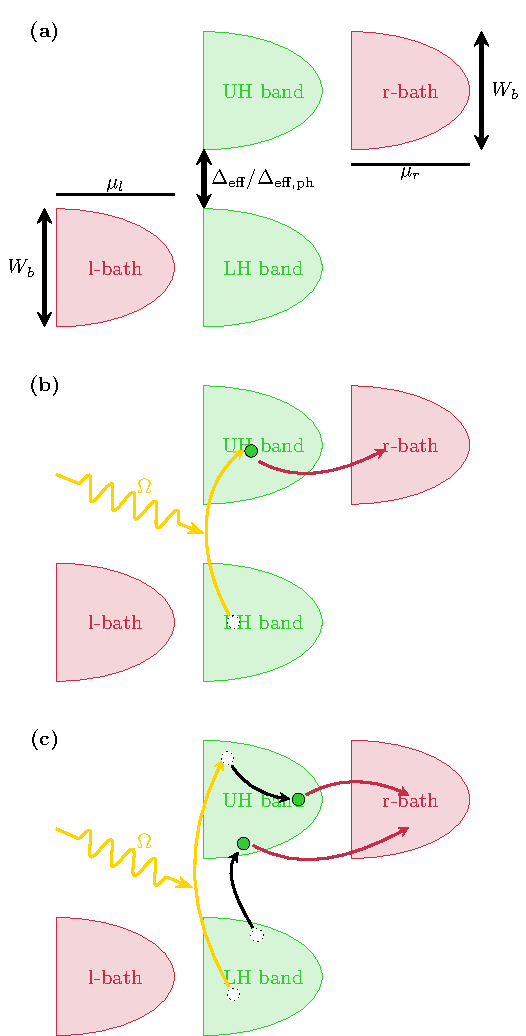
\includegraphics[width=0.9\linewidth]{./figures_Paper1/energy_setup.pdf}
\caption{(Colour online) Energy scheme and physical processes occuring in the considered setup. The baths bands are in red, the Hubbard bands in green and the vertical axis represents the energy. Panel (a) shows the quantities mentioned in Sec.\ref{sec:results}. Panel (b) illustrates a direct excitation process, in which an electron is excited  by a photon with energy $\Omega$ (yellow arrow) to the upper Hubbard band and escapes into the right bath (red arrow). Panel (c) displays an impact ionization process, where the photoexcited electron in the upper Hubbard band excites a second electron from the lower to the upper Hubbard band (black arrows) and they both escape into the right bath.}
\label{fig:energy_setup}
\end{figure}   

\subsection{Energy considerations and physical processes}
\label{sec:explicative_scheme}

We propose here a scheme, based on energy considerations, to describe the occurrence of impact ionization (IO) in our setup. We partially follow Ref.\cite{so.do.18,ma.ev.22} for the \emph{only-electron} case, extending it to the case with electron-phonon interaction. It holds at non-equilibrium steady state (NESS), where energy and particles conservation have to be respected and therefore no charge accumulation in the correlated layer is allowed.   

We assume that only first-order photon absorption processes occur. This is in fact the case for the chosen $\alpha$-values (see above) \cite{so.do.18}. We neglect also higher-order processes as multi-scattering IO processes. 

The essential condition to meet to have IO is that the bandwidth of the UHB is twice the effective gap $\Delta_{\textrm{eff}}$ \cite{so.do.18}. Only in this case, the photoexcited electron has enough energy to excite a second one across the gap. 

\subsubsection{Only electrons}
\label{sec:scheme_only_electrons}  
 
\begin{itemize}

\item For $\Omega<\Delta_{\textrm{eff}}$, we don't have any current if the DOS of the correlated layer has a true gap \footnote{To overcome the effective gap with $\Omega<\Delta_{\textrm{eff}}$ multiple-photon absorption processes should take place, but as written in the main text, such effects are negligible in the studied parameter range.}. If $\Delta_{\textrm{eff}}$ is a partial gap, we have a clear suppression of the current.  
 
\item For $\Delta_{\textrm{eff}}<\Omega<\Delta_{\textrm{eff}}+2W_b$, an electron coming from the left bath into the LHB is photoexcited to the UHB and can escape directly into the right bath without additional scattering (Fig.\ref{fig:energy_setup}(b)). From now on, we refer to such processes as direct excitations (DE). 
 
                             
\item For $2\Delta_{\textrm{eff}}<\Omega<\Delta_{\textrm{eff}}+2W_b$, a photoexcited electron in the UHB can excite via IO a second electron from LHB to the UHB, before being both dragged into the right bath (Fig.\ref{fig:energy_setup}(c)).

\item For $\Omega>\Delta_{\textrm{eff}}+2W_b$, there are no final states available for a photoexcited electron and the transition shouldn't occur. 

\end{itemize} 

From these considerations, we notice that in the energy window $\Delta_{\textrm{eff}}<\Omega<2\Delta_{\textrm{eff}}$ the only scattering processes taking place are DE, instead for $2\Delta_{\textrm{eff}}<\Omega<\Delta_{\textrm{eff}}+2W_b$ both DE and IO can occur. 

We point out that the boundaries of such energy ranges aren't strict and the separation of these physical processes can't be net, due to the influence of the various complicated mechanisms involved.

\subsubsection{Electron and phonons}
\label{sec:scheme_electrons_phonons}  
                            
With the inclusion of electron-phonon scattering, the outlined scheme remains valid except for the modification of the effective gap $\Delta_{\textrm{eff}}$. As shown in Sec.\ref{sec:E0_2_electrons_phonons}, the phonons broaden the DOS of the correlated layer and slightly close the gap. Therefore the effective gap is reduced by a small amount $\Delta_{\textrm{diss}}$ indicating the dissipation by phonons, i.e. $\Delta_{\textrm{eff,ph}}=\Delta_{\textrm{eff}}-\Delta_{\textrm{diss}}$.

\subsection{$E_0=2$}
\label{sec:E0_2}
  

\begin{figure*}[ht]
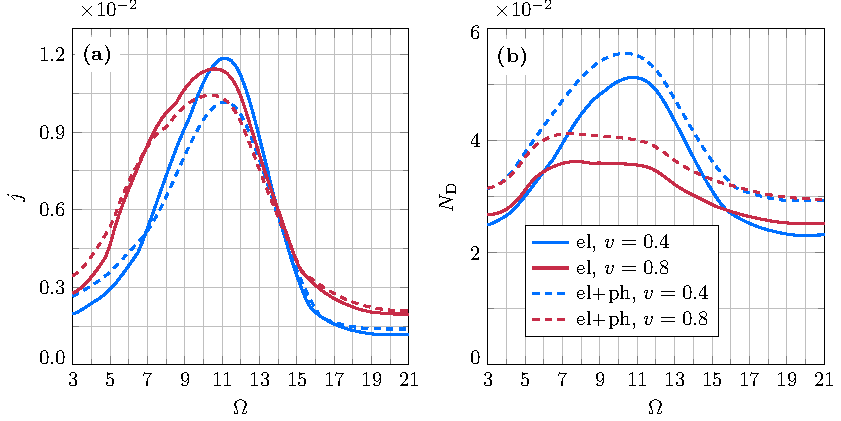
\includegraphics[width=\textwidth]{./figures_Paper1/j_vs_omega_mu1_v_0.4_0.8_eph.pdf}
% \captionsetup{width=\textwidth}
\caption{(Colour online) $\Omega$-dependence of time-averaged steady-state current $j$ (in units of $j_0=\frac{qt^*}{\hbar a^2}$) (a), double occupancy $N_D$ (b) and time-averaged current $j$ rescaled by $v^2$ (c), for $v=0.4$ and $v=0.8$, when electron-phonon interaction is switched off and on. The electron-phonon coupling is set to $g=0.8$ and the phonon cutoff frequency to $\omega_{ph}=0.1$. Default parameters are specified at the beginning of section~\ref{sec:results}.} 
\label{fig:j_vs_omega_mu1_v_0.4_0.8_eph}
\end{figure*}     
  

\subsubsection{Only electrons}
\label{sec:E0_2_only_electrons} 

\begin{figure}[ht] 
% \captionsetup{width=\textwidth} 
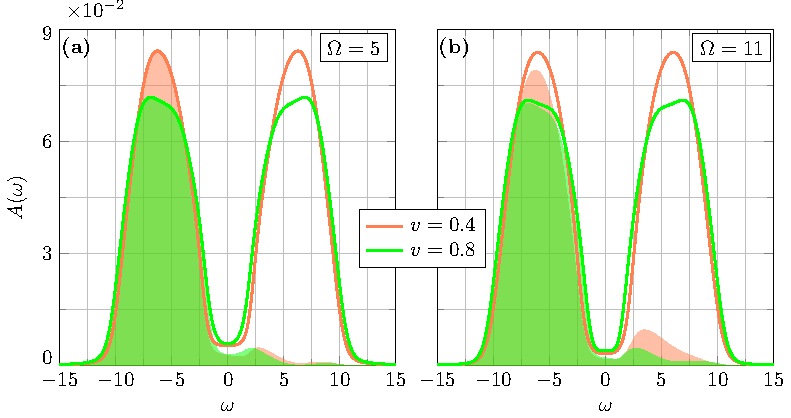
\includegraphics[width=\linewidth]{./figures_Paper1/spec_filling_mu1_v_0.4_0.8_O_5_11_e.pdf}
\caption{(Colour online) Spectral function $A(\omega)/t^{* -1}$ (solid) and occupation function $N(\omega)/t^{* -1}$ (shaded area), at $\Omega=5$ (a) and $\Omega=11$ (b) for $v=0.4,0.8$, when electron-phonon interaction is switched off. Default parameters are specified at the beginning of section~\ref{sec:results}.}
\label{fig:spec_filling_mu1_v_0.4_0.8_O_5_11_e}
\end{figure}  

We start from the analysis of the results obtained considering the electron-phonon interaction switched off, to describe the behaviour of the observables in terms of the bath-layer coupling $v$ only. 
 
In Fig.~\ref{fig:j_vs_omega_mu1_v_0.4_0.8_eph}(a) the photocurrent $j$ as a function of the driving frequency $\Omega$ shows an increase for both $v$ in the region $4\lesssim\Omega\lesssim8$ due to DE creating an electron-holon pair. Such range corresponds in fact, with our choice of parameters (see Sec.\ref{sec:results} and \ref{sec:scheme_only_electrons}), to the $\Omega$-region in which only DE can occur. For the same $\Omega$, $j_{v=0.8}>j_{v=0.4}$, clearly due to bigger value of $v$. In this region, the double occupation (Fig.~\ref{fig:j_vs_omega_mu1_v_0.4_0.8_eph}(b)) shows accordingly an increase for both $v$.
  
For $\Omega\gtrsim8$, the current increases further reaching for both $v$ its peak, located at $\Omega\approx 11$ \footnote{The position of the current peak roughly correspond to the resonant driving frequency $\Omega=U$.}. The magnitude of the peak is approximately the same for both $v$, despite the bath-layer couplings are one the double of the other. The double occupation in this region shows a similar behaviour for $v=0.4$, with a peak around $\Omega\approx 11$, while exhibits for $v=0.8$ a plateau. 

This region corresponds (see \ref{sec:scheme_only_electrons}) to the one in which both DE and IO can occur. Therefore what described above strongly suggests that for $v=0.4$ the dominant process taking place is IO, while for $v=0.8$ the dominant one is DE. In fact, for $v=0.4$ there is a clear increase in $N_D$ \footnote{
We point out that the increase of $N_D$ in Fig.\ref{fig:j_vs_omega_mu1_v_0.4_0.8_eph}, in comparison with Ref.\cite{so.do.18} isn't so steep and big in magnitude because in our setup choice, every photoexcited carrier can escape in the right bath.}, well-known signature for IO \cite{so.do.18,ma.ev.22} and the magnitude of the current peak is comparable with $v=0.8$: given the current formula Eq. \eqref{eq: Current furmula_00}, the prefactor $v^2$ for $v=0.4$ is four time smaller than the one for $v=0.8$, therefore such result should imply a different electronic scattering, as IO, doubling the number of carriers for a single photon absorption. On the other hand, the plateau in $N_D$ for $v=0.8$ means that a double occupation of a site doesn't increase with $\Omega$, signalizing that photoexcited electrons simply arrive in UHB and escape. An additional strong confirmation to such picture comes from Fig.~\ref{fig:j_vs_omega_mu1_v_0.4_0.8_eph}(c): the current $j$ rescaled by $v^2$ shows that the net contribution of the integral in $\eqref{eq: Current furmula_00}$ for $v=0.4$ is much bigger (roughly four times) than for $v=0.8$ and therefore the enhancement of the current has to come from a mutiplying-carriers electronic process.   

Such behaviour is extremely interesting: smaller $v$ means smaller probability amplitude of electrons entering in the LHB from the left bath and escaping from the UHB in the right bath. Despite that the magnitude of the photocurrent is roughly the same and IO process compensates almost completely this injection/drag deficency.  
 
The spectral features corroborate such hypotesis. In Fig.~\ref{fig:spec_filling_mu1_v_0.4_0.8_O_5_11_e}(a)-(b) the occupation function for $\Omega=5$, in the DE region, is almost the same for both $v$, while for $\Omega=11$ where the $j$-peak current occurs, the occupation of the UHB for $v=0.4$ is clearly bigger, in line with the peak of $N_D$.

Finally, increasing further $\Omega$ the current and double occupation decrease until they approach their minimum for $\Omega\approx20$ \footnote{The current $j$ doesn't go to zero as it should for $\Omega>20$ because of a background current intrinsic in the AMEA approach in presence of a gap or a band edge \cite{so.do.18}. This background current depends on $v$, $\mu_{l/r}$ and $g$, therefore we have different offsets according to the chosen parameters. Since we are interested in the qualitative behavior of the current and not stricly on the magnitude, we don't show these background currents, which don't affect our analysis.}.  
  

\subsubsection{Electrons and phonons}   
\label{sec:E0_2_electrons_phonons} 

\begin{figure}[ht]
% \captionsetup{width=\textwidth} 
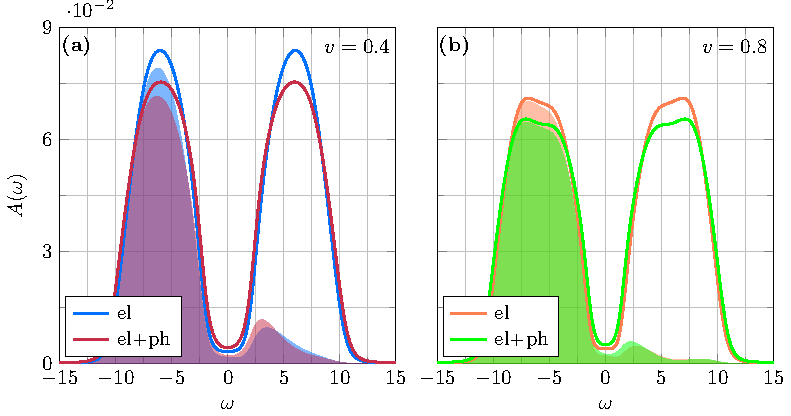
\includegraphics[width=\linewidth]{./figures_Paper1/spec_filling_mu1_v_0.4_0.8_O_11_eph.pdf}
\caption{(Colour online) Spectral function $A(\omega)/t^{* -1}$ (solid line) and occupation function $N(\omega)/t^{* -1}$ (dashed line) at $\Omega=11$ when electron-phonon interaction is switched off and on, for $v=0.4$ (a) and $v=0.8$ (b). The electron-phonon coupling is set to $g=0.8$ and the phonon cutoff frequency to $\omega_{ph}=0.1$. Default parameters are specified at the beginning of section~\ref{sec:results}.} 
\label{fig:spec_filling_mu1_v_0.4_0.8_O_11_eph}
\end{figure} 
 



We discuss now the effect of acoustic phonons on the results obtained in the previous section, switching on the electron-phonon coupling $g$. 
 
The current $j$ in presence of phonons in Fig.~\ref{fig:j_vs_omega_mu1_v_0.4_0.8_eph}(a) is slighty bigger than the \emph{only-electron} one for both $v$ when $\Omega\lesssim7$. This difference decreases increasing $\Omega$, until $\Omega\approx7$,  where a crossing takes place and the \emph{only-electron} current becomes bigger. Between $7\lesssim\Omega\lesssim14$, the current in presence of phonons follows the same behaviour of the \emph{only-electron} one, reaching for both $v$ its maximum, also located at $\Omega\approx 11$, but it shows a clear suppression in magnitude, occuring especially around the peak at $\Omega\approx 11$. For $\Omega\gtrsim14$ the current with phonons for both $v$ goes down until the minimum for $\Omega\approx20$ as before.

The double occupation $N_D$ with phonons (Fig.~\ref{fig:j_vs_omega_mu1_v_0.4_0.8_eph}(b)) for both $v$ remains bigger and follows the behaviour of the corresponding \emph{only-electron} counterpart within all the $\Omega$-range considered.


The spectral features including electron-phonon interaction shown in Fig.\ref{fig:spec_filling_mu1_v_0.4_0.8_O_11_eph} display a redistribution of the spectral weight towards the edges of the LHB and UHB, closing the gap and a suppression of the peaks of the bands. Consequently, the occupation of positive energy states is slightly shifted to the bottom of the UHB respect to the case without phonons, as the occupation function shows. The spectral function with phonons is then more broadened and tends to fill the effective gap $\Delta_{\textrm{eff}}$, as anticipated in Sec.\ref{sec:scheme_electrons_phonons}. 
 
Such feature explains why the current in presence of phonons in (Fig.~\ref{fig:j_vs_omega_mu1_v_0.4_0.8_eph}(a)) is slighty bigger in magnitude respect to the \emph{only-electron} one for both $v$ for $\Omega\lesssim7$. Such driving frequencies can excite across the gap only electrons coming from the upper edge of the LHB and due to $\Delta_{\textrm{eff,ph}}<\Delta_{\textrm{eff}}$, for the same $\Omega$ more photoexcited electrons end up in the UHB respect to the \emph{only-electron} case, with a consequent increase of the photocurrent. For example, Fig.\ref{fig:spec_filling_mu1_v_0.4_0.8_O_11_eph}(a)-(b) shows that an electron excited with $\Omega=4-5$ from the upper edge of the LHB ends close to the lower edge of UHB where $A(\omega)$ with phonons is slightly bigger than the \emph{only-electron} one.


We explain instead the suppression of the current with phonons respect to \emph{only-electron} one in the range $7\lesssim\Omega\lesssim14$, for both $v$, observing that for driving frequencies around the $j-$peak at $\Omega\approx 11$ the photoexcited electron in the UHB can come from three regions of LHB. Looking at Fig. \ref{fig:spec_filling_mu1_v_0.4_0.8_O_11_eph}(a)-(b), an electron can in fact be excited from the lower edge of LHB to lower edge of the UHB, from the middle of the LHB to the middle of UHB or from upper edge of LHB to the upper edge of the UHB. In the first and third case the electron comes and ends up in $\omega$-regions where the spectral function in presence of phonons has slightly more spectral weight than the \emph{only-electron} one, while in the second case the electron is excited between $\omega$-regions in which the \emph{only-electron} $A(\omega)$ is clearly bigger in magnitude than the one in presence of phonons. Overall, the dominant scattering process is the second one, yielding an higher current when only electrons are taken into account.

\pgcomm{Maybe this explanation above related to tunneling current} 
 
    
Regarding the trend of double occupation $N_D$ with phonons for both $v$ in Fig.~\ref{fig:j_vs_omega_mu1_v_0.4_0.8_eph}(b), we notice from Fig.\ref{fig:spec_filling_mu1_v_0.4_0.8_O_11_eph} that, for positive energies,  the occupation function in presence of phonons is almost always bigger than the \emph{only-electron} one. 

We discuss now the effect of phonons on DE/IO processes, as outlined in Sec.\ref{sec:E0_2_only_electrons}. 

The presence of phonons enhances slightly the current in almost all the region in which only DE take place (until $\Omega\lesssim7$, while the DE region ends at $\Omega\approx8$). They suppress the current in the range $7\lesssim\Omega\lesssim14$, where IO is the dominant electronic scattering process for $v=0.4$ and DE for $v=0.8$. This is confirmed by Fig.\ref{fig:j_vs_omega_mu1_v_0.4_0.8_E0_2_sweep_omegaph}, that shows that the effect of acoustic phonons on the observables is slightly boosted decreasing the soft cutoff phonon frequency $\omega_{ph}$, as the comparison with Fig.\ref{fig:j_vs_omega_mu1_v_0.4_0.8_eph} highlights \footnote{Decreasing $\omega_{ph}$, the acoustic phonon modes linear dispersion is always more truncated and increased in magnitude. Therefore the maximal value of the reciprocal lattice vector $\vec{q}_{\text{max}}$ such that $\omega_{\text{ph}}=\omega(\vec{q}_{\text{max}})$ \cite{ma.ga.22u} is reduced and consequently the dissipation by acoustic phonons is more effective.}. 
  
The results above suggest that the effect of acoustic phonons on the electronic scattering processes is the same, independently from their DE or IO origin, in fact they don't change drastically the interaction between the electrons. 
 
Moreover, their effect is independent of $v$, therefore independent of "how many" carriers are injected/dragged into/from the layer. Fig.\ref{fig:j_vs_omega_mu1_sweep_v_E0_2_eph} confirms such behaviour for the intermediate bath-layer couplings $v=0.5,0.6,0.7$, for which DE and IO at $\Omega\gtrsim8$ are even more mixed and hard to identify, together with their features \footnote{We don't consider smaller $v$ and smaller $E_0$ because they give a really slow convergence of DMFT loop. Moreover, the observables' magnitude becomes comparable with numerical fluctuations caused by numerical precision issues.}. 

\pgcomm{Are there some confirmations in literature regarding the effects of the phonons I observed?}

\begin{figure}[ht] 
% \captionsetup{width=\textwidth} 
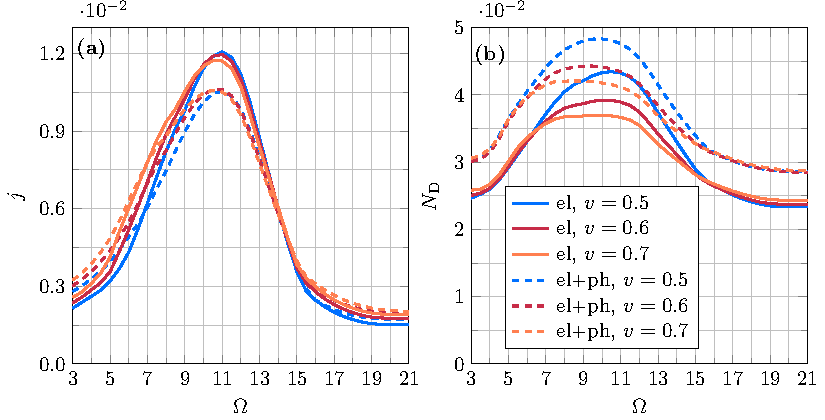
\includegraphics[width=\linewidth]{./figures_Paper1/j_vs_omega_mu1_sweep_v_E0_2_eph.pdf}
\caption{(Colour online) $\Omega$-dependence of time-averaged steady-state current $j$ (in units of $j_0=\frac{qt^*}{\hbar a^2}$) (a) and double occupancy $N_D$ (b), for $v=0.5,0.6,0.7$, when electron-phonon interaction is switched off and on. The electron-phonon coupling is set to $g=0.8$ and the phonon cutoff frequency to $\omega_{ph}=0.1$. Default parameters are specified at the beginning of section~\ref{sec:results}.} 
\label{fig:j_vs_omega_mu1_sweep_v_E0_2_eph}
\end{figure} 
 

\begin{figure}[ht] 
% \captionsetup{width=\textwidth} 
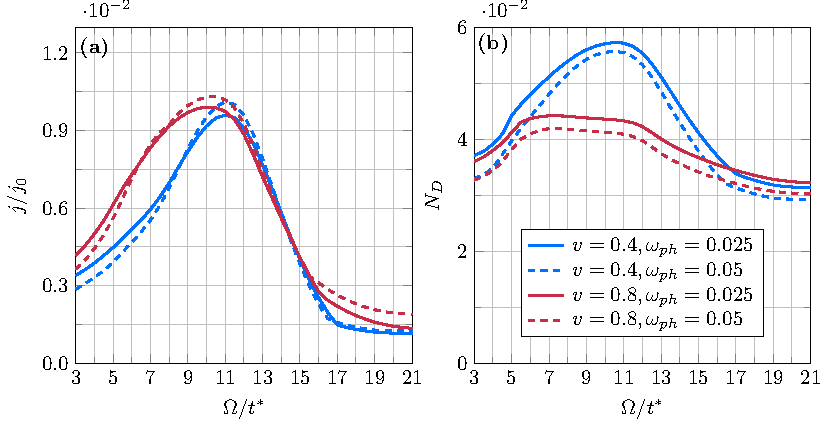
\includegraphics[width=\linewidth]{./figures_Paper1/j_vs_omega_mu1_v_0.4_0.8_E0_2_sweep_omegaph.pdf}
\caption{(Colour online) $\Omega$-dependence of time-averaged steady-state current $j$ (in units of $j_0=\frac{qt^*}{\hbar a^2}$) (a) and double occupancy $N_D$ (b), for $v=0.4,0.8$, at  phonon cutoff frequencies $\omega_{ph}=0.025,0.05$. The electron-phonon coupling is set to $g=0.8$. Default parameters are specified at the beginning of section~\ref{sec:results}.} 
\label{fig:j_vs_omega_mu1_v_0.4_0.8_E0_2_sweep_omegaph}
\end{figure} 
 

\newpage

\subsection{Higher $E_0$}
\label{sec:higher_E0}


\begin{figure*}[ht] 
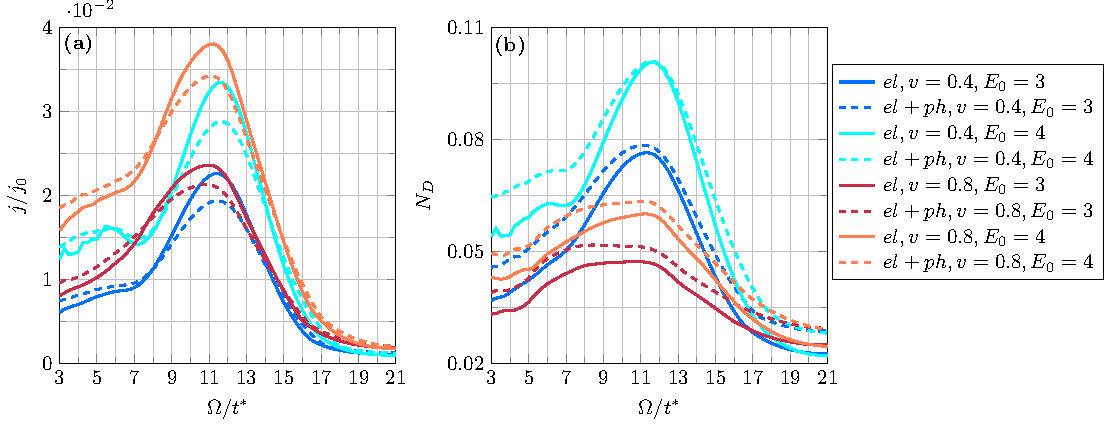
\includegraphics[width=\textwidth]{./figures_Paper1/j_vs_omega_mu1_v_0.4_0.8_eph_E0_3_4.pdf}
% \captionsetup{width=\textwidth}
\caption{(Colour online) $\Omega$-dependence of time-averaged steady-state current $j$ (in units of $j_0=\frac{qt^*}{\hbar a^2}$) (a) and double occupancy $N_D$ (b), for $v=0.4,0.8$ at different electric field amplitudes $E_0=3,4$, when electron-phonon interaction is switched off and on. The electron-phonon coupling is set to $g=0.8$ and the phonon cutoff frequency to $\omega_{ph}=0.1$. Default parameters are specified at the beginning of section~\ref{sec:results}.} 
\label{fig:j_vs_omega_mu1_v_0.4_0.8_eph_E0_3_4}
\end{figure*}     

\subsubsection{Only electrons}
\label{sec:higher_E0_only_electrons} 
 
As for Sec.\ref{sec:E0_2_only_electrons}, we analyze first the results obtained without the electron-phonon interaction.

The trend of the current as a function of $\Omega$ for the two different $v$ at increasing $E_0$ in Fig.\ref{fig:j_vs_omega_mu1_v_0.4_0.8_eph_E0_3_4}(a) follows the one outlined in Sec. \ref{sec:E0_2_only_electrons}. 

For both $E_0=3,4$ the current maximum, located around $\Omega\approx11.5$, is due mainly to IO for $v=0.4$ and mainly to DE for $v=0.8$, as the double occupation in Fig.\ref{fig:j_vs_omega_mu1_v_0.4_0.8_eph_E0_3_4}(b) clearly shows. These results are in accordance with Sec.\ref{sec:E0_2_only_electrons}. This is confirmed also by Fig.\ref{fig:spec_filling_mu1_v_0.4_0.8_E3_4_O_11.5_e}(a)-(b) in which is evident the bigger occupation of the UHB for $v=0.4$. 
 
There are however some features to be discussed more in detail.

The magnitude of the current clearly increases with $E_0$ and there is a steeper increase of $j$ in the $\Omega$-region after $\Omega\approx8$ for both $v$ respect to $E_0=2$ (Fig.\ref{fig:j_vs_omega_mu1_v_0.4_0.8_eph}). The current peak for $v=0.8$ becomes bigger than the corresponding one for $v=0.4$ increasing the electric field amplitude $E_0$. A small bump develops at $E_0=4$ for $v=0.4$ around $\Omega\approx6$. Its position, directly in the middle of DE region (Sec.\ref{sec:scheme_only_electrons}) suggests an origin due to DE \cite{so.do.18}.  

\pgcomm{The position of the current peaks seem to have a linear dependence on $E_0$. (see mail). Putting here the plots would have taken really long time and maybe we don't even insert this part.}  

Also the double occupation as a function of $\Omega$ for the two $v$ at increasing $E_0$ in Fig.\ref{fig:j_vs_omega_mu1_v_0.4_0.8_eph_E0_3_4}(b) follows the one outlined in Sec. \ref{sec:E0_2_only_electrons}. However, the magnitude of $N_D$ is enhanced clearly with $E_0$, especially the $N_D$ peaks for $v=0.4$, in comparison with the $E_0=2$ case in Fig.\ref{fig:j_vs_omega_mu1_v_0.4_0.8_eph}(b). Moreover, the difference in $N_D$ between the two $v$ at the same $E_0$ increases with $E_0$, as Fig.\ref{fig:spec_filling_mu1_v_0.4_0.8_E3_4_O_11.5_e} also shows. 

Therefore, increasing $E_0$, we have an overall enhancement of the photocurrent and of double occupation. The current for $v=0.8$ in which DE play a major role is enhanced respect to the one $v=0.4$ coming mainly from IO. However, the latter experiences an extreme increase in both the observables $j$ and $N_D$, confirmed by Fig.\ref{fig:spec_filling_mu1_v_0.4_0.8_E3_4_O_11.5_e}. 


\begin{figure}[ht]
% \captionsetup{width=\textwidth} 
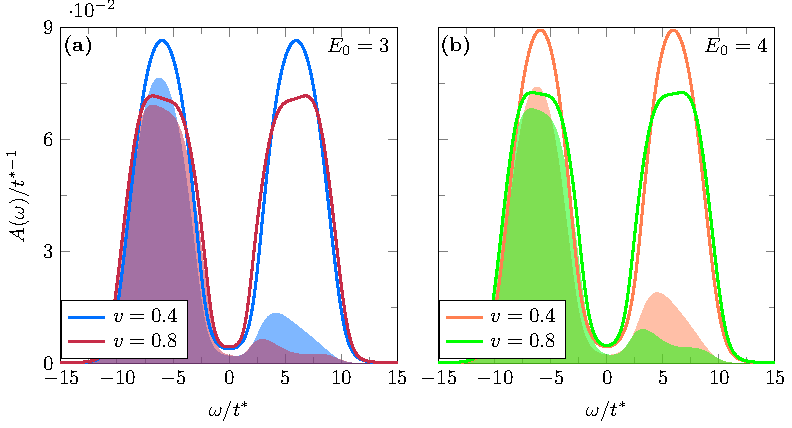
\includegraphics[width=\linewidth]{./figures_Paper1/spec_filling_mu1_v_0.4_0.8_E3_4_O_11.5_e.pdf}
\caption{(Colour online) Spectral function $A(\omega)/t^{* -1}$ (solid line) and occupation function $N(\omega)/t^{* -1}$ (shaded area) at $\Omega=11.5$ for $v=0.4,0.8$ when electron-phonon interaction is switched off, for $E_0=3$ (a) and $E_0=4$ (b). Default parameters are specified at the beginning of section~\ref{sec:results}.} 
\label{fig:spec_filling_mu1_v_0.4_0.8_E3_4_O_11.5_e}
\end{figure} 

\subsubsection{Electrons and phonons}
\label{sec:higher_E0_electrons_phonons} 

As in Sec.\ref{sec:E0_2_electrons_phonons}, we discuss now the results obtained including the acoustic phonons.

The $\Omega$-dependence of the current with phonons respect to the \emph{only-electron} one follows for both $v$ and $E_0$ the behaviour outlined in Sec.\ref{sec:E0_2_electrons_phonons}, with two minor differences, namely the crossing between the currents with and without phonons, occurring in this case at $\Omega\approx8$ and the current peaks slighly shifted at $\Omega\approx11.5$. For the small bump at $E_0=4$, $v=0.4$ around $\Omega\approx6$ there is no difference whether the phonons are taken into account or not.

 
The double occupation $N_D$ with phonons (Fig.~\ref{fig:j_vs_omega_mu1_v_0.4_0.8_eph_E0_3_4}(b)) for both $v$ and $E_0$ is bigger and goes like the corresponding \emph{only-electron} one over all the $\Omega$-range, similarly to Sec.\ref{sec:E0_2_electrons_phonons}.

However, for increasing $E_0$, the $N_D$-peak in presence of phonons for $v=0.4$, around $\Omega\approx11.5$, is clearly flattened on the relative \emph{only-electron} one. There is this tendency (even though really small) also for $v=0.8$. 

The spectral features with the electron-phonon interaction remain the same as described in Sec.\ref{sec:E0_2_electrons_phonons}(see Fig.\ref{fig:spec_filling_mu1_v_0.4_0.8_O_11_eph}). 
  
 
The effect of phonons on DE/IO processes as $E_0$ is increased is the same as discussed in Sec.\ref{sec:E0_2_electrons_phonons}. Overall, as Fig.\ref{fig:j_vs_omega_mu1_v_0.4_0.8_eph_E0_3_4}(a)-(b) show, their effect is independent of the electric field amplitude $E_0$, therefore independent of "how strong" electrons are driven from the external AC field. 

\section{Conclusions}
\label{sec:conclusions} 
  
We investigated the influence of fermion baths and phonons dissipation on electron transport and spectral properties of a Mott insulating layer driven to the non-equilibrium
steady state by an external AC field. In order to reproduce a possible Mott-based photovoltaic setup between metallic leads, we considered partially filled wide-band fermion baths, addressing the issue regarding how acoustic phonons dissipate the energy carried by photoexcited electrons. We demonstrated the importance of the coupling to fermion baths on the electron scattering process occurring at different driving frequencies and observed how the dissipation by phonons influences the photocurrent and the double occupation. We found a strong evidence that the dominant electron scattering mechanism responsible for the photocurrent peak is impact ionization at small couplings to the fermion baths, almost absent at higher couplings. Higher electric field amplitudes substantially boost the photocurrent and the double occupation, without modifying the picture above. Acoustic phonons dissipation slightly boosts the photocurrent for small driving frequencies and suppresses it at higher ones, in correspondence to the peak, disregarding the dominant electron scattering process taking place. Phonons effect isn't influenced from the bath-layer coupling value and the electric field amplitude.

 
These results suggest that in correlated layers weakly coupled to single layers or quantum dots, in turn connected to metallic leads, impact ionization may occur significantly. From the experimental point of view, such realization is employed, for example, to bridge semiconductor quantum dots to reservoirs through small molecules \cite{wa.mc.13,wa.bo.17}, to extract hot photoexcited carriers \cite{ti.ke.10,ca.wa.16}. 

A positive aspect towards the future research in this direction is that a moderate electron-phonon coupling doesn't seem to suppress drastically the current, as our results show, and therefore in real materials, impact ionization might contribute consistently to overcome the Schockley-Queisser limit \cite{sh.qu.61}.  
 
However, in order to address the occurrence of impact ionization in realistic setups, one should take into account the feedback of the electrons on the phonon dynamics with a self-consistent treatment and the effect of impurities scattering. Another step forward would be the extension to multiorbital systems \cite{pe.be.19} in a multilayer setup, to model oxide heterostructures \cite{as.bl.13,pe.be.19}, where the correlated region is made of multiple layers and photoexcited carriers are separated via an electric field gradient.

 
%  For electric field amplitudes in the sunlight range the generated photocurrent, even though small, could yield an efficiency exploitable for some applications. On the the other side, for experimental setups or scientific-based devices, a strong AC electric field, realized with a more concentrated light source like laser, would give a much bigger photocurrent with a broader range of future applications.


% In second instance, such model misses still some ingredients as impurities/defects scatterings, long-range Coulomb effects, a multilayer structure with an intrinsic electric field gradient separating the charges. All these additional elements are present in Mott materials as oxide heterostructures proposed as a prototype for Mott solar cells. At the present level there's no point in considering now such features towards a more realistic description, because all these additional ingredients would complicate and hide the basic mechanisms still to be clarified completely.
 
\section*{Acknowledgements}
This work was supported by the Austrian Science Fund (FWF) within Project P 33165-N, as well as NaWi Graz. The computational results presented have been obtained using the Vienna Scientific Cluster (VSC) and the D-Cluster Graz.
 
     
      
   
\bibliographystyle{prsty}   
% references in Phys Rev style
\bibliography{footnotes,references_database}
 
% \bibliographystyle{/afs/itp.tugraz.at/user/arrigoni/noneq-group/bibtex/prsty} 
%\bibliography{New_References,/afs/itp.tugraz.at/user/arrigoni/noneq-group/bibtex/references_database.bib}
% \bibliography{Additional_Refs.bib,references_database.bib}
%\bibliography{New_References,references_database.bib}

\end{document}  
